\chapter{Sistemi lineari} 

\begin{figure}[h]
    \centering
    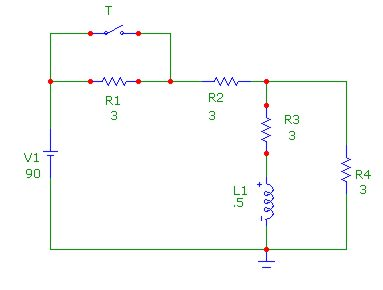
\includegraphics[scale = 1]{esempio di sistema lineare.jpeg}
\end{figure}  

\newpage 

\section{Cosa è un sistema lineare e cosa rappresenta} 

È detto sistema lineare un sistema descritto da un'equazione integro-differenziale 
lineare, che leghi un segnale di ingresso x(t) (detto anche sollecitazione) 
al corrispondente segnale in uscita (o risposta) y(t). \newline 

Se l'equazione integro-differenziale è a coefficienti costanti, 
il sistema risulta invariante nel tempo (detto anche sistema permanente). \newline 

Il problema fondamentale consiste nel determinare l'evoluzione dell'uscita y(t) a partire dalla conoscenza 
dell'ingresso x(t). \newline 

{
    \begin{figure}[h]
        \centering
        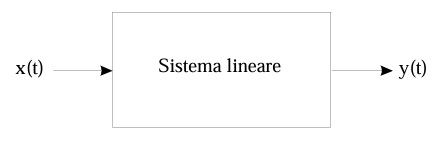
\includegraphics[scale = 1]{Blocco sistema lineare.PNG}
    \end{figure}  
     
}

Il problema consiste nel descrivere opportunatamente il blocco lineare intermedio e nel mettere in relazione 
le due funzioni x(t) e y(t). \newline 

I sistemi lineari sono molto comodi perchè, grazie al principio della sovrapposzione, 
è possibile sapere y(t) come combinazione lineare di $y_1(t)$ e $y_2(t)$, che, rispettivamente, 
sono le uscite dei segnali di ingresso $x_1(t)$ e $x_2(t)$. \newline 

Grazie alla proprietà di campionamento della delta di Dirac, possiamo scrivere che: 

{
    \Large 
    \begin{equation}
        x (t) 
        = 
        \int_{- \infty}^{+ \infty} 
        x (\tau) \delta(t - \tau) d\tau
    \end{equation}
}

Questa formula ci spiega che x(t) può essere vista come somma di un'infinità non numerabili di impulsi matematici 
$\delta (t - \tau)$ disposti in $t = \tau$ di area pari a $x(\tau) d\tau$, $\tau$ varia da $[-\infty, +\infty]$. \newline 

Indichiamo con h(t) la risposta del sistema ad un impulso matematico in $t=0$, cioè: 

{
    \Large 
    \begin{equation}
        y(t) = h(t) \leftrightarrow x(t) = \delta(t)
    \end{equation}
}

Se il sistema è permanente, la risposta ad un impulso matematico allocata in $t = \tau$ sarà $h(t - \tau)$. \newline 

Grazie al principio della sovrapposzione degli effetti, possiamo scrivere che: 

{
    \Large 
    \begin{equation}
        y(t) = \int_{-\infty}^{+\infty}
        x(\tau) h (t - \tau) d\tau
    \end{equation}
}

y(t) esprime la relazione ingresso-uscita ed è chiaramente un integrale di convoluzione. \newline 

Quindi possiamo applicare tutte le proprietà che abbiamo visto nei capitoli precedenti. \newline 

Possiamo esprimere la risposta impulsiva di un sistema come: 

{
    \Large 
    \begin{equation}
        y(t) = x(t) * h(t)
    \end{equation}
}

\begin{tcolorbox}
Nel corso degli appunti, $\otimes$  o * saranno segni interscambiali per indicare una convoluzione tra i segnali     
\end{tcolorbox}

Come visto nella convoluzione, è conveniente esprimere e fare i calcoli in frequenza piuttosto che nel tempo. \newline 

La trasformata dell'uscita y(t) sarà: 

{
    \Large 
    \begin{equation}
        Y(\omega) = X(\omega)H(\omega) 
    \end{equation}
}

in cui $Y(\omega)$,  $X(\omega)$ e $H(\omega)$ sono rispettivamente le trasformate di Forurier 
dell'uscita, dell'ingresso e della risposta impulsiva del sistema. \newline 

Sapendo $Y(\omega)$ è possibile riportare l'uscita nel dominio del tempo, anti-trasformando $Y(\omega)$: 

{
    \Large 
    \begin{equation}
        y (t)= F^{-1} [Y(\omega)] = F^{-1} [X(\omega) H(\omega) ] 
    \end{equation}
}

La funzione $H(\omega)$ prende il nome di funzione di trasferimento del sistema. \newline 

$H(\omega)$ modifica lo spettro del segnale di ingresso, eliminando parte dello spettro originale: 
ecco perchè un sistema lineare viene definito anche come filtro. \newline 

Idealmente, le frequenze che passano nel filtro non sono modificate dal sistema-lineare, 
nella realtà ci saranno alcune modifiche. \newline 


Quindi, possiamo dividere i filtri in due categorie: 

\begin{itemize}
    \item filtri fisicamente realizzabili 
    \item filtri idealmente realizzabili 
\end{itemize} 

In un filtro vero, vale a dire costruito con componenti reali, la risposta non può precedere la sollecitazione. \newline 

Sapendo che h(t) è la risposta impulsiva in $t=0$, ciò comporta che, in un filtro "vero" debba essere: 

{
    \Large 
    \begin{equation}
        h(t) = 0 \text{ per } t < 0 
    \end{equation}
} 

Questa proprietà va sotto il nome di principio di causalità e rappresenta la condizione necessaria affinche
un filtro idealmente lo sia anche fisicamente. \newline 

\newpage 


\section{Densità spettrale di energia e di potenza in un filtro} 

Essendo: 

{
    \Large 
    \begin{equation}
        Y(\omega) = H(\omega) X(\omega)
    \end{equation}
}

le densità spettrali di energia (ove applicabili) dei segnali in ingresso e in uscita sono tra 
loro legate dalla seguente relazione: 

{
    \Large 
    \begin{equation}
        \abs{Y(\omega)} ^{2} 
        = 
        \abs{H(\omega) X(\omega)} ^{2} 
        = 
        \abs{H(\omega)} ^{2} \cdot \abs{X(\omega)} ^{2}
    \end{equation}
}

Una relazione analoga vale per gli spettri di potenza, indicati con $p_x (\omega)$ 
(per l'ingresso) e $p_y (\omega)$ (per l'uscita): 

{
    \Large 
    \begin{equation}
        p_y (\omega) = \abs{H(\omega)} ^{2} p_x (\omega)
    \end{equation}
}

Dunque, la densità in uscita si ottiene moltiplicando la densità in ingresso 
per il modulo al quadrato della funzione di trasferimento. \newline 

Sapendo la relazione tra densità spettrale e funzione di auto-correlazione di un segnale, possiamo 
conoscere la relazione ingresso-uscita anche nel dominio del tempo. \newline 

Anti-trasformando $\abs{Y(\omega)} ^{2}$ e $p_y (\omega)$ otteniamo che: 

{
    \Large 
    \begin{equation}
        R_y (\tau) 
        = 
        \int_{-\infty}^{+ \infty}
        R_h (t) R_x (\tau - t) dt  
    \end{equation}
}

dove: 

{
    \Large 
    \begin{equation}
        R_h (\tau) = h(t) * h^{*} (-t)
    \end{equation}
}

ovvero la funzione auto-correlazione della risposta impulsiva del sistema .\newline 

\newpage 

\section{Il problema della distorsione} 

Come detto precedemente, il sistema lineare può causare delle distorsioni nello spettro. \newline 

Un sistema lineare può solo togliere e/o mantenere parte dello spettro, non può aggiungere: 
in questo ultimo caso, il sistema viene definito non lineare. \newline 

Ci sono diversi tipi di distorsioni, quelli che andremo ad analizzare sono i seguenti. \newline 

\begin{itemize}
    \item Distorsione lineare 
    \item Distorsione non lineare 
    \item Distorsione causata da percorsi multipli 
    \item Canali con fading
\end{itemize} 

\newpage 

\subsection{Distorsione lineare} 

Per un dato sistema lineare, ad esempio un canale di trasmissione, un ingresso x(t) produce 
un'uscita y(t) viene "processato" secondo le seguenti caratteristiche. \newline 

Supponiamo lo spettro del segnale di ingresso come: 

{
    \Large 
    \begin{equation}
        X(\omega) = \abs{X(\omega)} e^{\jmath \theta_x (\omega)}
    \end{equation}
}

e la funzione di trasferimento del sistema: 

{
    \Large 
    \begin{equation}
        H(\omega) = \abs{H(\omega)} e^{\jmath \theta_h (\omega)}
    \end{equation}
}

Allora, facendo la convoluzione nel tempo tra le due funzioni di trasferimento, 
quindi una moltiplicazione in $\omega$, avremo che: 

{
    \Large 
    \begin{equation}
        \begin{split}
            Y(\omega) 
            &= 
            X(\omega) H(\omega) 
            \\ 
            &= \abs{X(\omega)} e^{\jmath \theta_x (\omega)} \cdot \abs{H(\omega)} e^{\jmath \theta_h (\omega)} 
            \\ 
            &= \abs{X(\omega)} \cdot \abs{H(\omega)} e^{\jmath [\theta_x (\omega) + \theta_h (\omega)]}
        \end{split}
    \end{equation}
}

Dall'ultima equazione, notiamo che, attraverso il sistema lineare, lo spettro di ampiezza di 
$x(t)$ viene moltiplicato per il modulo della funzione di trasferimento e lo spettro di fase 
di $x(t)$ viene aumentato della fase della funzione di trasferimento. \newline 

Quindi, il segnale di uscita presenta, in genere, uno spettro diverso da quello del segnale di ingresso 
e risulta, rispetto a x(t), distorto, quindi diverso. \newline 

Se si tratta di un sistema di comunicazione, generalmente, questa distorsione è voluta, 
ma, generalmente, non lo è. \newline 

Possiamo introdurre delle condizioni di non distorsione.\newline 

Il segnale risulta non distorto se viene amplificato o attenuato. \newline 

Considerando: 

{
    \Large 
    \begin{equation}
        y(t) = A x(t)
    \end{equation}
}

il segnale di ingresso viene moltiplicato se $A > 1$, viene attenuato se $A < 1$. \newline 

Inoltre, un'altra condizione per cui il segnale risulta non essere distorto se il segnale 
$x(t)$ risulta ritardato di un tempo costante $t_d$: 

{
    \Large 
    \begin{equation}
        y(t) = A x(t - t_d)
    \end{equation}
}

Nei sistemi reali, il ritardo è "fisiologico" in quanto legato al tempo di propagazione, 
e in certi casi ai tempi di elaborazione. \newline 

In assenza di distorsione, tutte le componenti del segnale di ingresso devono raggiungere 
l'uscita indistorte, mantenendo cioè i loro rapporti relativi. \newline 

In altri termini, significa che tutte le componenti in frequenza devono subire la stessa amplificazione o la stessa attenuazione. \newline 

Ciò implica che: 

{
    \Large 
    \begin{equation}
        \abs{H(\omega)} = A
    \end{equation}
}

Inoltre, per non avere distorsione, tutte le componenti in frequenza devono raggiungere l'uscita con lo stesso ritardo $t_d$. \newline 

Ad esempio, per un segnale cosinusoidale: 

{
    \Large 
    \begin{equation}
        \cos(\omega t) \text{ con ritardo $t_d$} 
        \rightarrow 
        \cos[\omega (t - t_d)] = \cos(\omega t -\omega t_d)
    \end{equation}
}

Da questa breve dimostrazione, si conclude che un ritardo $t_d$ comporta una variazione di fase 
pari a $\omega t_d$. \newline 

Si conclude che, per un ritardo temporale $t_d$, la varazione di fase è proporzionale alla pulsazione $\omega$. \newline 

Se $H(\omega)$ sia responsabile di un ritardo costante per tutte le componenti 
armoniche che l'attraversano, la sua fase deve essere proporzionale a $\omega$. \newline 

Quindi: 

{
    \Large 
    \begin{equation}
        \theta_h (\omega) = -\omega t_d
    \end{equation}
}

Da tutte queste ossservazioni, si nota che, per non avere distorsioni $H(\omega)$ deve essere: 

{
    \Large 
    \begin{equation}
        H(\omega) = A e^{\jmath \omega t_d}
    \end{equation}
}

quindi, la trasformata di Forurier del segnale di uscita, sarà: 

{
    \Large 
    \begin{equation} 
        \begin{split}
            Y(\omega) 
            &= X(\omega) H(\omega) 
            \\ 
            &= X(\omega) A e^{\jmath \omega t_d} 
            \\ 
            &= A X(\omega) e^{\jmath \omega t_d}
        \end{split} 
    \end{equation}
}

Riassumento, esplicitando modulo e fase di $H(\omega)$, 
le condizioni di non distorsione lineare di un sistema  sono le seguenti: 

{
    \Large 
    \begin{equation}
        \begin{cases}
            \abs{H(\omega)} = A \\ 
            \theta_h (\omega) = -\omega t_d  
        \end{cases}
    \end{equation}
} 

Teoricamente, le condizioni appena citate dovrebbero valere per ogni pulsazione da 
$[-\infty, + \infty]$. \newline 

Nella pratica, considerando un filtro reale, queste condizioni saranno vere in una determinata banda del filtro, 
che possiamo nominare come $[-\omega_{mx}, +\omega_{mx}]$. \newline 

Un esempio dello spettro di un filtro reale: 

{
    \begin{figure}[h]
        \centering
        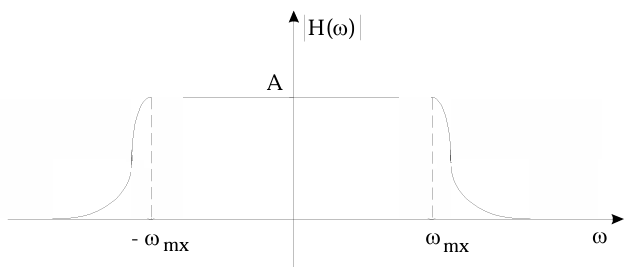
\includegraphics[scale = 0.5]{Spettro dei moduli di un filtro lineare.PNG}
    \end{figure}  
     
}


{
    \begin{figure}[h]
        \centering
        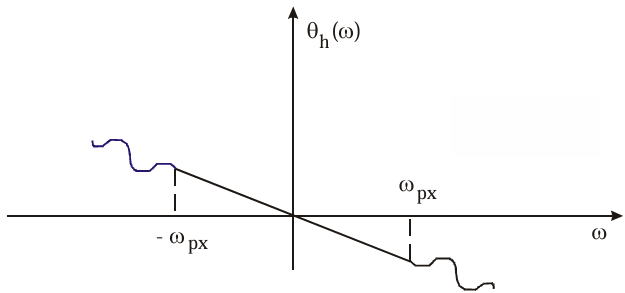
\includegraphics[scale = 0.5]{Spettro delle fasi di un filtro lineare.PNG}
    \end{figure}  
     
} 

\newpage  


Praticamente, tutti i mezzi trasmissivi utilizzati nei sistemi di comunicazione presentano 
un comportamento passa-basso, e dunque eliminano le componenti ad alta frequenza del segnale che li attraversa. \newline 

Le componenti ad alta frequenza sono responsabili delle transizioni veloci. \newline 

Quindi, il segnale filtrato è costretto ad assumere un andamento più "smussato". \newline 

Definiamo come dispersione il meccanismo di allargamento nel tempo del segnale. \newline 

Gli effetti della dispersione sono particolarmente dannosi nelle trasmissioni numeriche, 
dove il segnale trasmesso è costituito da una sequenza di impulsi. \newline 

{
    \begin{figure}[h]
        \centering
        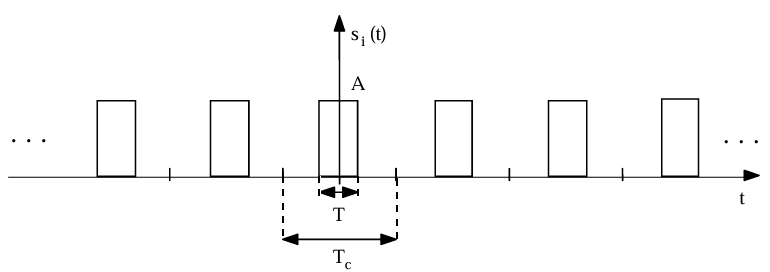
\includegraphics[scale = 0.75]{Treno di impulsi.PNG} 
        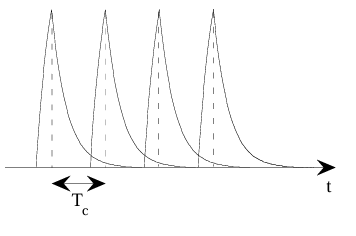
\includegraphics[scale = 0.75]{Treno di impulsi filtrato.PNG}
    \end{figure}  
     
}

Le due figure mostrano, in alto, il segnale di ingresso, in basso, il segnale filtrato. \newline 

Dalla figura del treno di impulsi filtrato, notiamo che la coda del generico impulso si sovrappone 
agli impulsi successivi, determinando il fenomeno denominato "interferenza di intersimbolo" (o ISI). \newline 

Oltre ai filtri passa-basso, esistono anche i filtri passa-alto, che, a differenza dei filtri passa-basso, 
fanno passare le frequenze ad alta frequenza, non lasciando passare le frequenze a bassa frequenza. \newline 

Nella realtà, questi filtri non esistono, sono un'astrazione puramente matematica. \newline 

Nella realtà, oltre ai filtri-passa basso, avremo i filtri passa-banda (che a sua volta sono formati 
da due filtri passa-basso) che, come dicono il nome, fanno passare le componenti in frequenza di una certa banda. \newline 

Generalmente, nei mezzi trasmissivi e negli apparati ad essi collegati, il canale di trasmissione, oltre 
a bloccare la componente continua, $\omega = 0$, elimina le componenti ad alta frequenza, $\omega > \omega_{px}$. \newline 

Dunque, la migliore modellazione di un sistema di comunicazione è quella di un filtraggio passa-banda. \newline 

\newpage 

\subsection{Distorsione non lineare} 

La proprietà di linearità di un dato sistema non è indipendete dal segnale di ingreso. \newline 

Il comportamento lineare vale sotto l'potesi di applicazione di (relativamente) piccoli segnali. \newline 

Quando l'ampiezza della sollecitazione diventa elevata, 
una descrizione accurata del sistema non può più prescindere dalle non linearità. \newline 

Quando l'ipotesi di piccoli segnali non può essere ritenuta valida, le non linearità devono 
essere introdotte nella descrizione del sistema e ne modificano significativamente la caratterizzazione. \newline 

Ci sono delle differenze rispetto alla distorsione lineare. \newline 

Il legame ingresso-uscita nel dominio del tempo non può più essere descritto da un integrale di convoluzione: 
è necessario specificare puntualmente il valore assunto dall'uscita in corrispondenza di un dato valore all'ingresso. \newline 

Supponendo che il legame sia instantaneo (sistema non lineare senza memoria), 
la caratteristica che lega il segnale di uscita y(t) a quello di ingresso x(t) può essere espressa come: 

{
    \Large 
    \begin{equation}
        y(t) = f[x(t)]
    \end{equation}
} 

dove f è una funzione generica non lineare. \newline 

Se f è una funzione non lineare, y(t) possiamo esprimerlo con lo sviluppo in serie di Mac-Laurin come: 

{
    \Large 
    \begin{equation}
        y(t) 
        =
        a_0 + a_1 x(t) + a_2 x^{2} (t) + a_3 x^{3} (t) + .... + a_k x^{k} (t) + ...
    \end{equation}
}

Se y(t) è composto dai coeffiecienti $a_0$ e/o $a_1$, allora possiamo dire che y(t) è legato 
linearmente da x(t), se y(t) è composto da coefficienti maggiori di uno, allora y(t) è legato 
da x(t) da una relazione non lineare. \newline 

A causa della loro non linearità, per i sistemi non lineari non è definibile una funzione di trasferimento. \newline 

Per i sistemi non lineari, dovremo svolgere k convoluzioni per quanti sono i coeffcienti dello sviluppo in serie di 
Mac-Laurin di y(t). \newline 

\newpage 

\subsection{Distorsione causata da percorsi multipli} 

Una trasmissione a percorsi multipli (in inglese Multipath) ha 
luogo quando il segnale trasmesso arriva al ricevitore seguendo due o più percorsi caratterizzati da ritardi differenti. \newline 

Uno schema di quello che succede, ad esempio, in una trasmissione radio: 

\begin{figure}[h]
    \centering
    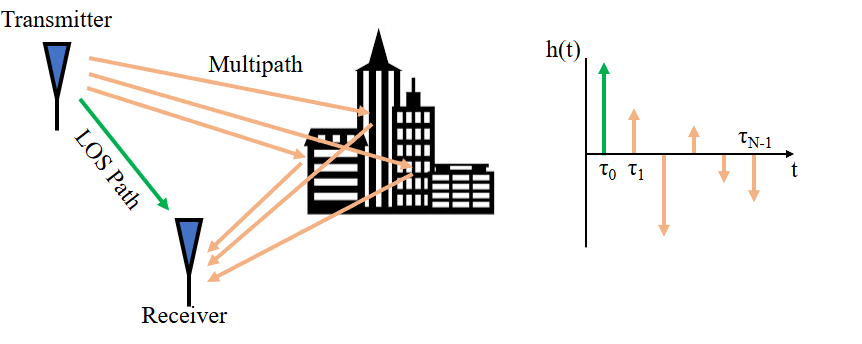
\includegraphics[scale = 0.6]{Multipath IRL.PNG}
\end{figure} 

In presenza di percorsi multipli, il canale può essere schematizzato mediante più canali in parallelo, ciascuno con differente attenuazione relativa e differente 
ritardo temporale. \newline 

{
    \begin{figure}[h]
        \centering
        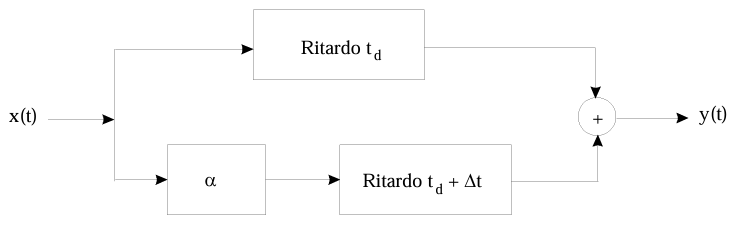
\includegraphics[scale = 1]{Esempio di multipath.PNG} 
    \end{figure}  
     
}

La seguente figura è un esempio di multipath con due soli percorsi: 
\begin{itemize}
    \item uno con guadagno unitario e ritardato di $t_d$ 
    \item l'altro con guadagno $\alpha$ e ritardato di $t_d + \Delta t$
\end{itemize}  

Tipicamente, $\alpha < 1$: in questo caso si tratta, propriamente, di un'attenuazione; 
se $\alpha > 1$ si tratta di amplificazione, me generalemente ciò non capita nel multipath. \newline  

Se consideriamo questo multipath, in frequenza, considerando i due cammini, avremo che: 

{
    \Large 
    \begin{equation}
        \begin{cases}
            H_1 (\omega) = e^{-\jmath \omega t_d} \\ 
            H_2 (\omega) = \alpha e^{-\jmath \omega (t_d + \Delta t)} 
        \end{cases}
    \end{equation}
} 

Quindi, la funzione di trasfermineto dell'intero sistema è: 

{
    \Large 
    \begin{equation}
        \begin{split}
            H(\omega) 
            &= 
            H_1 (\omega) + H_2 (\omega) 
            \\ 
            &= 
            e^{-\jmath \omega t_d} +  \alpha e^{-\jmath \omega (t_d + \Delta t)} 
            \\ 
            &= 
            e^{-\jmath \omega t_d} (1 + \alpha e^{-\jmath \omega \Delta t}) 
            \\
            {
                \small
                \text{Applicando la formula di Eulero }
            }
            &= 
            e^{-\jmath \omega t_d} 
            [1 + \alpha \cos(\omega \Delta t) - \jmath \alpha \sin(\omega \Delta t)] 
            \\ 
            &= 
            \sqrt{1 + \alpha ^{2} + 2 \alpha \cos(\omega \Delta t)} 
            \cdot 
            e^{-\jmath [\omega t_d + \arctan \frac{\alpha \sin(\omega \Delta t)}{1 + \alpha \cos(\omega \Delta t)}]}
        \end{split}
    \end{equation}
}

Si può concludere che la trasmissione multipath dà luogo ad una funzione di trasferimento non ideale (sia nell'ampiezza che nella fase) 
ed è quindi responsabile di una particolare distorsione lineare. \newline 

In quanto tale, tale distorsione può essere almeno parzialmente corretta con l'uso di equilizzatori. \newline 

{
    \begin{figure}[h]
        \centering
        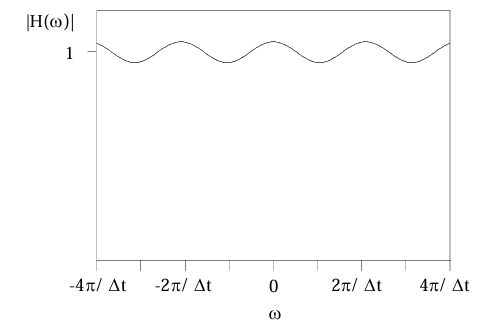
\includegraphics[scale = 0.5]{Esempio di multipath modulo.PNG}
        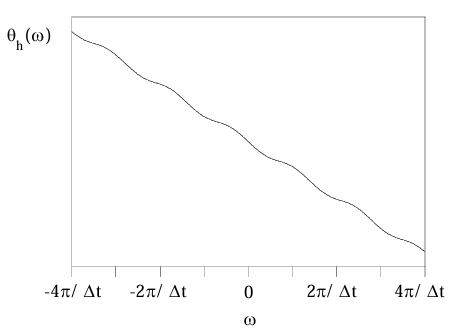
\includegraphics[scale = 0.5]{Esempio di multipath fase.PNG}  
    \end{figure}  
     
} 
\newpage 

\subsection{Canali con fading}

Fino ad ora abbiamo assunto le caratteristiche del canale costanti nel tempo. \newline 

Tuttavia, nella pratica e nella vita reale, molti canali di trasmissione presentano proprietà variabili nel tempo. \newline 

Il canale cambierà le sue proprietà nel tempo. \newline

Perciò, la funzione di trasferimento del canale varia a sua volta nel tempo in maniera aleatoria, causando attenuazione pure aleatorie 
(o random in inglese) del segnale. \newline 

Questo tipo di fenomeno è noto come fading. \newline 

\newpage 
.
\newpage
. 
\newpage
